\documentclass[10pt]{article}  

%%%%%%%% PREÁMBULO %%%%%%%%%%%%
\title{Reporte de Laboratorio}
\usepackage[spanish]{babel} %Indica que escribiermos en español
\usepackage[utf8]{inputenc} %Indica qué codificación se está usando ISO-8859-1(latin1)  o utf8  
\usepackage{amsmath} % Comandos extras para matemáticas (cajas para ecuaciones,
% etc)
\usepackage{amssymb} % Simbolos matematicos (por lo tanto)
\usepackage{longtable} %agregadom para hacer tablas
\usepackage{xltabular}
\usepackage{tabularray}
\usepackage{graphicx} % Incluir imágenes en LaTeX
\usepackage{emptypage}
\usepackage{color} % Para colorear texto
\definecolor{Blanco}{gray}{1}
\definecolor{Gray}{rgb}{0.501,0.501,0.501}
\definecolor{Tranquil}{rgb}{0.89,1,1}

\usepackage{subfigure} % subfiguras
\usepackage{float} %Podemos usar el especificador [H] en las figuras para que se
% queden donde queramos
\usepackage{capt-of} % Permite usar etiquetas fuera de elementos flotantes
% (etiquetas de figuras)
\usepackage{sidecap} % Para poner el texto de las imágenes al lado
\sidecaptionvpos{figure}{c} % Para que el texto se alinie al centro vertical
\usepackage{caption} % Para poder quitar numeracion de figuras
\usepackage{commath} % funcionalidades extras para diferenciales, integrales,
% etc (\od, \dif, etc)
\usepackage{cancel} % para cancelar expresiones (\cancelto{0}{x})
 
\usepackage{anysize} 					% Para personalizar el ancho de  los márgenes
\marginsize{2cm}{2cm}{2cm}{2cm} % Izquierda, derecha, arriba, abajo

\usepackage{appendix}
\renewcommand{\appendixname}{Apéndices}
\renewcommand{\appendixtocname}{Apéndices}
\renewcommand{\appendixpagename}{Apéndices} 
% Para que las referencias sean hipervínculos a las figuras o ecuaciones y
% aparezcan en color
\usepackage[colorlinks=true,plainpages=true,citecolor=blue,linkcolor=blue]{hyperref}
%\usepackage{hyperref} 
% Para agregar encabezado y pie de página
\usepackage{fancyhdr} 
\pagestyle{fancy}
\fancyhf{}
\fancyhead[L]{\footnotesize UNI} %encabezado izquierda
\fancyhead[R]{\footnotesize Fac. de Ciencias}   % dereecha
\fancyfoot[R]{\footnotesize Reporte}  % Pie derecha
\fancyfoot[C]{\thepage}  % centro
\fancyfoot[L]{\footnotesize Segunda Ley de Newton}  %izquierda
\renewcommand{\footrulewidth}{0.4pt}

\usepackage{listings} % Para usar código fuente
\definecolor{dkgreen}{rgb}{0,0.6,0} % Definimos colores para usar en el código
\definecolor{gray}{rgb}{0.5,0.5,0.5} 
% configuración para el lenguaje que queramos utilizar
\lstset{language=Matlab,
   keywords={break,case,catch,continue,else,elseif,end,for,function,
      global,if,otherwise,persistent,return,switch,try,while},
   basicstyle=\ttfamily,
   keywordstyle=\color{blue},
   commentstyle=\color{red},
   stringstyle=\color{dkgreen},
   numbers=left,
   numberstyle=\tiny\color{gray},
   stepnumber=1,
   numbersep=10pt,
   backgroundcolor=\color{white},
   tabsize=4,
   showspaces=false,
   showstringspaces=false}

\newcommand{\sen}{\operatorname{\sen}}	% Definimos el comando \sen para el seno
%en español

\title{Plantilla para Reportes IMEC-UTB}
% Basada en la plantilla para reportes UPIITA de  Overleaf

%%%%%%%% TERMINA PREÁMBULO %%%%%%%%%%%%

\begin{document}

%%%%%%%%%%%%%%%%%%%%%%%%%%%%%%%%%% PORTADA %%%%%%%%%%%%%%%%%%%%%%%%%%%%%%%%%%%%%%%%%%%%
																					%%%
\thispagestyle{empty}
\begin{center}																		%%%
\newcommand{\HRule}{\rule{\linewidth}{0.5mm}}									%%%\left
 																					%%%

\hspace{0.9cm}

\textsc{\huge Universidad Nacional de Ingeniería }\\[0.8cm]
			
\textsc{\LARGE Facultad de Ciencias}

\vspace{0.6cm}



\includegraphics[scale = 0.15]{Imagenes/UNI.png}

													 								%%%
\vspace*{0.6cm}								%%%
																					%%%	



\begin{minipage}{0.9\textwidth} 
\begin{center}																					%%%
\textsc{\LARGE  Laboratorio de Física BFI01 A\\[0.7cm] Reporte 05}
\end{center}
\end{minipage}\\[0.3cm]
%%%
    																				%%%
 			\vspace*{0.4cm}																		%%%
																					%%%
\HRule \\[0.5cm]																	%%%
{ \huge \bfseries Principio de Arquímedes}\\[0.2cm]	%%%
 																					%%%
\HRule \\[0.9cm]																	%%%
 																				%%%
																					%%%
\begin{minipage}{0.46\textwidth}													%%%
\begin{flushleft} \large															%%%

% Aqui a continuación pongan los nombres de los integrantes
\emph{El grupo conformado por:}\\[2mm]
Llactahuaman Quispe Benjamin\\20232268G \\[1mm]
Cortez Núñez Christian\\20232203B\\[1mm]
Rocca Cruz Axel\\20234046A\\[1mm]
 

%%%
			%\vspace*{2cm}	
            													%%%
										 						%%%
\end{flushleft}																		%%%
\end{minipage}		
																%%%
\begin{minipage}{0.52\textwidth}		
\vspace{-1.9cm}											%%%
\begin{flushright} \large															%%%
\emph{Profesor:}\\[2mm]																	%%%
Tello Gálvez Julio César\\[1mm]Brocca Pobes Manuel Enrique\\
\end{flushright}																	%%%
\end{minipage}	
\vspace*{1cm}
%\begin{flushleft}
 	
%\end{flushleft}
%%%																	%%%															
\vspace{-2.4cm}	
\begin{minipage}{0.98\textwidth}
\begin{flushright}	
\large
\emph{Fecha de la práctica:}\\
\vspace{0.2cm}
26 de mayo de 2023 
\end{flushright}
\end{minipage}

 \vspace{2.4cm}

\large{\today}\\
\vspace{0.3cm}

{ \Large\bfseries 2023-1}
										 			
\end{center}							 											
																					
\newpage																		
%%%%%%%%%%%%%%%%%%%% TERMINA PORTADA %%%%%%%%%%%%%%%%%%%%%%%%%%%%%%%%

\tableofcontents 
\setcounter{page}{1}


\newpage


\begin{center}
    \textbf{\huge Principio de Arquímedes}
\end{center}

\section{Objetivos}
\subsection{Competencias Generales}
\begin{itemize}
    \item Determinar la masa de tres cuerpos a partir del torque que produce su peso
    \item Determinar la densidad media de algunos cuerpos mediante la aplicación del Principio de Arquímedes
\end{itemize} 

\subsection{Competencias Específicas}
\begin{itemize}
    \item Utiliza una balanza de brazos con contrapeso para hallar la masa de un cuerpo y el empuje que se produce sobre dicho cuerpo al estar sumergido.

\end{itemize}

\section{Datos obtenidos}

\subsection{Peso de los cuerpos}

\begin{figure}[H]
    \begin{center}
        \caption{Cuerpo 1 (Cilindro Plomo)} {\label{fig:plomo}} 
        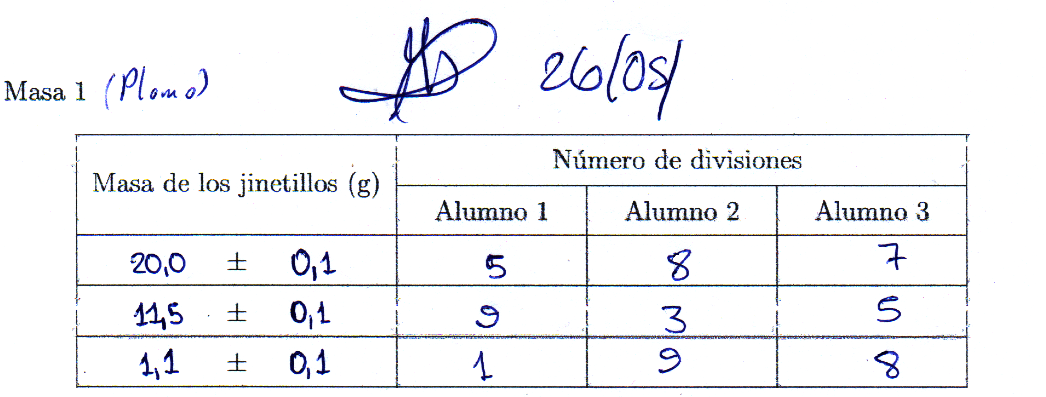
\includegraphics[width = 0.78\textwidth]{Imagenes/Peso Final 1.png}
    \end{center}

    \vspace{-0.1cm}
    \begin{center}
        \caption{Cuerpo 2 (Cilindro dorado)}  {\label{fig:laton}} 
        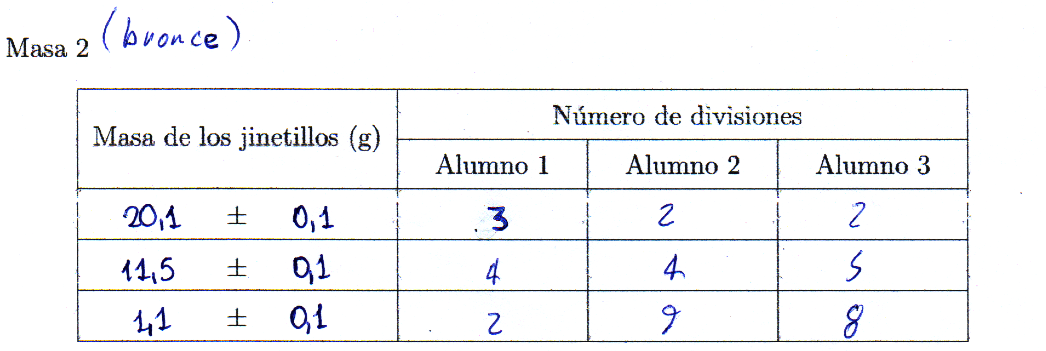
\includegraphics[width = 0.78\textwidth]{Imagenes/Peso Final 2.png}
    \end{center}
\end{figure}

\newpage
\begin{figure}[H]
    \begin{center}
        \caption{Cuerpo 3 (Esfera blanca)}  {\label{fig:blanco}} 
        \vspace{-0.3cm}
        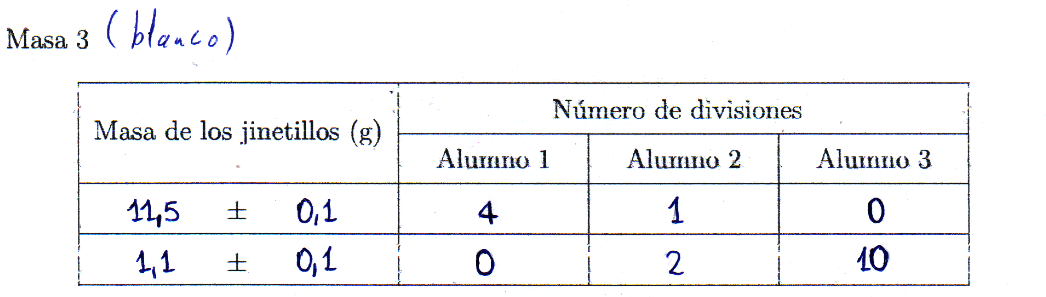
\includegraphics[width = 0.78\textwidth]{Imagenes/Peso Final 3.png}
    \end{center}
\end{figure}

\vspace{-0.8cm}

\subsection{Peso aparente de los cuerpos sumergidos en agua}
\vspace{-0.1cm}
\begin{figure}[H]
    \begin{center}
        \caption{Cuerpo 1 (Cilindro plomo)}  {\label{fig:plomo en agua}} 
        \vspace{-0.3cm}
        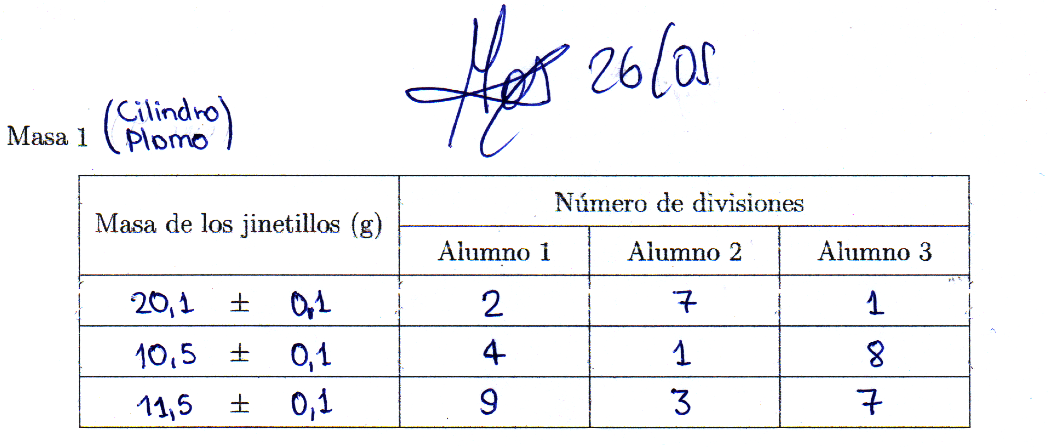
\includegraphics[width = 0.78\textwidth]{Imagenes/Peso Aparente 1.png}
        
        \vspace{0.4cm}
        \caption{Cuerpo 2 (Cilindro dorado)}  {\label{fig:laton en agua}} 
        \vspace{-0.3cm}
        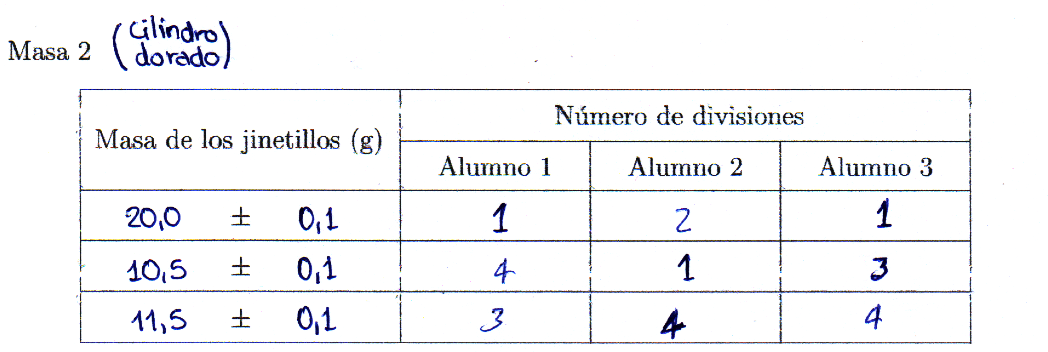
\includegraphics[width = 0.78\textwidth]{Imagenes/Peso Aparente 2.png}
        
        \vspace{0.5cm}
        \caption{Cuerpos 1 y 3 (Esfera blanca + Cilindro plomo)}  {\label{fig:blanco y plomo en agua}}
        \vspace{-0.1cm}
        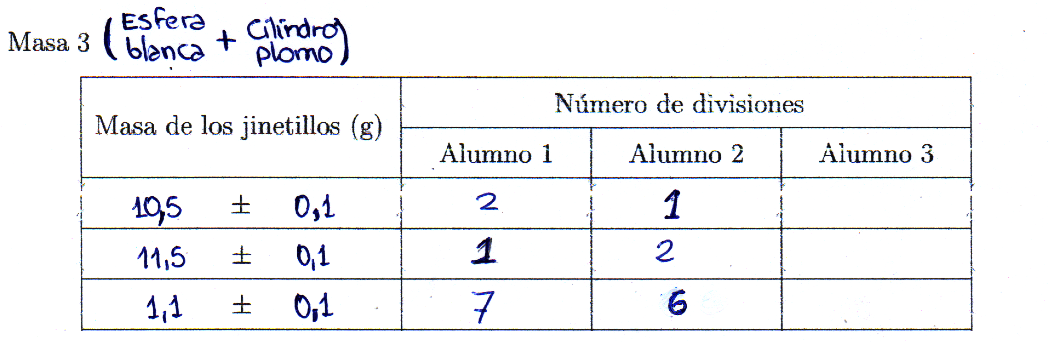
\includegraphics[width = 0.78\textwidth]{Imagenes/Peso Aparente 3.png}
    \end{center}
\end{figure}

\section{Cálculos y resultados}

\subsection{Cálculo de la masa de los cuerpos}\vspace{2mm}

Uso de los siguientes recursos:    
\begin{itemize}
    
    \item Figuras \ref{fig:plomo}, \ref{fig:laton} y           \ref{fig:blanco}
    
    \item Constantes y asunciones:
        \begin{itemize}
            \item Distancia D = 10 u (la última división)
            \item Las distancias son exactas (no incertidumbre)
        \end{itemize}
    
    \item Fórmulas:
    \large
    {\begin{equation}
        \label{masa}
        Masa = \frac{\Sigma~(masa_{i} \times distancia_{i})}{D}
    \end{equation}
    \vspace{-0.1cm}
    \begin{equation}
        \label{delta masa}
        \Delta Masa =\frac{\Sigma~(\Delta masa_{i} \times distancia_{i})}{D}
    \end{equation}}
\end{itemize}

\vspace{-0.2cm}
\subsubsection{Cuerpo 1 (Cilindro Plomo):}
\vspace{0,2cm}

Completamos 3 veces las ecuaciones \ref{masa} y \ref{delta masa}, de acuerdo a la figura \ref{fig:plomo}:\\

Cálculo de masa:

\begin{equation*} 
    Masa = \frac{(20\times5)+(11,5\times9)+(1,1\times1)}{10} = 21~g
\end{equation*}
\begin{equation*}
    Masa = \frac{(20\times8)+(11,5\times3)+(1,1\times9)}{10} = 20~g
\end{equation*}
\begin{equation*}
    Masa = \frac{(20\times7)+(11,5\times5)+(1,1\times8)}{10} = 20~g
\end{equation*}
\vspace{0.2cm}
\begin{equation*}
    \textbf{Masa~promedio}= \frac{21+20+20}{3} = \textbf{20~g}
\end{equation*}
\vspace{0.1cm}

Cálculo de la incertidumbre:
\begin{equation*}
     \Delta Masa =\frac{(0,1\times5)+(0,1\times9)+(0,1\times1)}{10} = 0,2~g
\end{equation*}
\begin{equation*}
     \Delta Masa =\frac{(0,1\times8)+(0,1\times3)+(0,1\times9)}{10} = 0,2~g
\end{equation*}
\begin{equation*}
     \Delta Masa =\frac{(0,1\times7)+(0,1\times5)+(0,1\times8)}{10} = 0,2~g
\end{equation*}
\vspace{0.2cm}
\begin{equation*}
    \Delta \textbf{Masa~promedio} = \frac{0,2+0,2+0,2}{3} = \textbf{0,2~g}
\end{equation*}

\vspace{0.3cm}
\begin{center}
    \textbf{Masa del cilindro plomo = 20,5 $\pm$ 0,2 g}
\end{center}

\subsubsection{Cuerpo 2 (Cilindro Dorado):}
\vspace{0,2cm}

Completamos 3 veces las ecuaciones \ref{masa} y \ref{delta masa}, de acuerdo a la figura \ref{fig:laton}:\\

Cálculo de masa:

\begin{equation*} 
    Masa = \frac{(20\times3)+(11,5\times4)+(1,1\times2)}{10} = 11~g
\end{equation*}
\begin{equation*}
    Masa = \frac{(20\times2)+(11,5\times4)+(1,1\times9)}{10} = 9,6~g
\end{equation*}
\begin{equation*}
    Masa = \frac{(20\times2)+(11,5\times5)+(1,1\times8)}{10} = 10,6~g
\end{equation*}
\vspace{0.2cm}
\begin{equation*}
    \textbf{Masa~promedio}= \frac{11+9,6+10,6}{3} = \textbf{10,4~g}
\end{equation*}
\vspace{0.1cm}

Cálculo de la incertidumbre:
\begin{equation*}
     \Delta Masa =\frac{(0,1\times3)+(0,1\times4)+(0,1\times2)}{10} = 0,09~g
\end{equation*}
\begin{equation*}
     \Delta Masa =\frac{(0,1\times2)+(0,1\times4)+(0,1\times9)}{10} = 0,2~g
\end{equation*}
\begin{equation*}
     \Delta Masa =\frac{(0,1\times2)+(0,1\times5)+(0,1\times8)}{10} = 0,2~g
\end{equation*}
\vspace{0.2cm}
\begin{equation*}
    \Delta \textbf{Masa~promedio} = \frac{0,09+0,2+0,2}{3} = \textbf{0,2~g}
\end{equation*}

\vspace{0.3cm}
\begin{center}
    \textbf{Masa del cilindro dorado = 10,0 $\pm$ 0,2 g}
\end{center}
\vspace{0.1cm}

\subsubsection{Cuerpo 3 (Esfera blanca):}
\vspace{0,2cm}

Completamos 3 veces las ecuaciones \ref{masa} y \ref{delta masa}, de acuerdo a la figura \ref{fig:blanco}:\\

Cálculo de masa:

\begin{equation*} 
    Masa = \frac{(11,5\times4)+(1,1\times0)}{10} = 4,6~g
\end{equation*}
\begin{equation*}
    Masa = \frac{(11,5\times1)+(1,1\times2)}{10} = 1,4~g
\end{equation*}
\begin{equation*}
    Masa = \frac{(11,5\times0)+(1,1\times10)}{10} = 1,1~g
\end{equation*}
\vspace{0.2cm}
\begin{equation*}
    \textbf{Masa~promedio}= \frac{4,6+1,4+1,1}{3} = \textbf{2~g}
\end{equation*}
\vspace{0.1cm}

Cálculo de la incertidumbre:
\begin{equation*}
     \Delta Masa =\frac{(0,1\times4)+(0,1\times0)}{10} = 0,04~g
\end{equation*}
\begin{equation*}
     \Delta Masa =\frac{(0,1\times1)+(0,1\times2)}{10} = 0,03~g
\end{equation*}
\begin{equation*}
     \Delta Masa =\frac{(0,1\times0)+(0,1\times10)}{10} = 0,1~g
\end{equation*}
\vspace{0.2cm}
\begin{equation*}
    \Delta \textbf{Masa~promedio} = \frac{0,09+0,15+0,15}{3} = \textbf{0,06~g}
\end{equation*}

\vspace{0.3cm}
\begin{center}
    \textbf{Masa de la esfera blanca = 2 $\pm$ 0,06 g}
\end{center}
\vspace{0.3cm}

\subsection{Cálculo del volumen sumergido en el agua}
\vspace{2mm}

Uso de los siguientes recursos:    
\begin{itemize}
    
    \item Figuras \ref{fig:plomo en agua}, \ref{fig:laton en agua} y           \ref{fig:blanco y plomo en agua}
    
    \item Constantes y asunciones:
        \begin{itemize}
            \item Densidad del agua $\rho_{agua}$ = 1 g/ml
            \item Gravedad g = 9,81 m/s$^{2}$
            \item Distancia D = 10 u (la última división)
            \item Las distancias son exactas (no incertidumbre)
        \end{itemize}
    
    \item Fórmulas:
    \large
    {\begin{equation}
        \label{tension}
        Peso~aparente = Tensi\Acute{o}n_{~cuerda}= \frac{\Sigma~(masa_{i} \times distancia_{i})~g}{D}
    \end{equation}
    \vspace{-0.1cm}
    \begin{equation*}
        Tensi\Acute{o}n_{~promedio} + Empuje = Masa_{~promedio} \times g 
    \end{equation*}
    \vspace{-0.2cm}
    \begin{equation}
        \label{volumen}
        Volumen = \frac{Masa_{~promedio} - T}{\rho_{agua}} 
    \end{equation}}
\end{itemize}

\subsubsection{Cuerpo 1 (Cilindro Plomo):}
\vspace{0,2cm}

Completamos 3 veces las ecuaciones \ref{tension} y \ref{volumen}, de acuerdo a la figura \ref{fig:plomo en agua}:\\

\begin{equation}
    T = \frac{(20,1\times2)+(10,5\times4)+(11,5\times9)}{10}\times9,81
\end{equation}


\newpage
    


\begin{table}[H]
\centering
\begin{tblr}{
  cells = {c},
  cell{2}{1} = {r=5}{},
  cell{8}{4} = {Gray},
  cell{8}{5} = {Gray},
  cell{8}{6} = {Gray},
  hline{1,9} = {-}{0.1em},
  hline{2,7-8} = {-}{},
}
Variables & x     & y     & xy    & x$^{2}$ & y$^{2}$\\
Datos     & 0,001 & 0,202 & 0,000 & 0,000 & 0,041  \\
          & 0,022 & 0,707 & 0,016 & 0,000 & 0,500  \\
          & 0,048 & 1,687 & 0,081 & 0,002 & 2,846  \\
          & 0,092 & 2,848 & 0,262 & 0,008 & 8,111  \\
          & 0,137 & 4,017 & 0,550 & 0,019 & 16,136 \\
Sumatoria & 0,300 & 9,461 & 0,909 & 0,030 & 27,634 \\
\end{tblr}
\end{table}

\vspace{0,2cm}
Reemplazando en las ecuaciones 1, 2 y 3 obtenemos:

\begin{equation*}
    \Bar{x} = \frac{0,300}{5} = \textbf{0,060} \textcolor{Blanco}{.............} \Bar{y} = \frac{9,461}{5} = \textbf{1,892}
\end{equation*}
\vspace{0,1cm}
\begin{equation*}
    m = \frac{5\times0,909-0,300\times9,461}{5\times0,030 - (0,300)^{2}} = \textbf{28,399} 
\end{equation*}
\vspace{0,1cm}
\begin{equation*}
    b = 1,892 - 28,399\times0,060 = \textbf{0,188}
\end{equation*}

\vspace{-0.5cm}
\begin{center}
\textbf{La ecuación de la recta hallada es: $y = 28,399x + 0,188$}\\[0,3cm]

\textbf{La constante elástica del resorte A es: 28,399 N/m}
\end{center}

\hspace{1cm}


\subsubsection{Resorte B (0,081 m):}
\vspace{0,2cm}

Formamos la siguiente tabla de datos:
\begin{table}[H]
\centering
\begin{tblr}{
  cells = {c},
  cell{2}{1} = {r=5}{},
  cell{8}{4} = {Gray},
  cell{8}{5} = {Gray},
  cell{8}{6} = {Gray},
  hline{1,9} = {-}{0.1em},
  hline{2,7-8} = {-}{},
}
Variables & x     & y     & xy    & x$^{2}$ & y$^{2}$\\
Datos     & 0,001 & 0,202 & 0,000 & 0,000 & 0,041  \\
          & 0,004	& 0,707	& 0,003	& 0,000	& 0,500  \\
          & 0,027 & 1,687	& 0,046	& 0,001	& 2,846  \\
          & 0,066	& 2,856	& 0,188	& 0,004	& 8,157  \\
          & 0,104 & 4,017	& 0,418	& 0,011	& 16,136 \\
Sumatoria & 0,202 &	9,469 & 0,655 & 0,016 &27,680 \\
\end{tblr}
\end{table}

\vspace{0,2cm}
Reemplazando en las ecuaciones 1, 2 y 3 obtenemos:

\begin{equation*}
    \Bar{x} = \frac{0,202}{5} = \textbf{0,040} \textcolor{Blanco}{.............} \Bar{y} = \frac{9,469}{5} = \textbf{1,894}
\end{equation*}
\vspace{0,1cm}
\begin{equation*}
    m = \frac{5\times0,655-0,202\times9,469}{5\times0,016 - (0,202)^{2}} = \textbf{35,102} 
\end{equation*}
\vspace{0,1cm}
\begin{equation*}
    b = 1,894 - 35,102\times0,040 = \textbf{0,476}
\end{equation*}

\vspace{-0,7cm}
\begin{center}
\textbf{La ecuación de la recta hallada es: $y = 35,102x + 0,476$}\\[0,3cm]
\textbf{La constante elástica del resorte A es: 35,102 N/m}
\end{center}

\newpage
\hspace{1cm}


\subsection{Módulo de la Fuerza resultante en tres puntos}\vspace{2mm}

Uso de los siguientes recursos:
\begin{itemize}
    \item Datos de la Tabla 1
    \item Ecuaciones de las rectas A y B anteriores
    \item Fórmula de Fuerza Resultante:
    \large{\begin{equation}
        F_{R} = \sqrt{F^{2}_{A} + F^{2}_{B} + 2(F_{A} \times F_{B} \times cos \alpha)}
    \end{equation}}
\end{itemize}

\vspace{0,2cm}
Hallamos las fuerzas F$_{A}$,F$_{B}$ y la F$_{R}$  para cada punto:

Punto 18:
 \begin{equation*}
    F_{A} = 28,399 \times (0,243) + 0,188 = 7,089
    \textcolor{Blanco}{--------------}
\end{equation*}
\begin{equation*}
    F_{B} = 35,102 \times (0,031) + 0,476 = 1,564
    \textcolor{Blanco}{--------------}
\end{equation*}  
\begin{equation*}
    F_{R} = \sqrt{(7,089)^{2} + (1,564)^{2} + 2(7,089 \times 1,564 \times cos(1,99)} = \textbf{6,609 N}
\end{equation*}
\vspace{-0,2cm}

Punto 22:
 \begin{equation*}
    F_{A} = 28,399 \times (0,239) + 0,188 = 6,975
    \textcolor{Blanco}{-------------..-}
\end{equation*}
\begin{equation*}
    F_{B} = 35,102 \times (0,071) + 0,476 = 2,968
    \textcolor{Blanco}{--------------}
\end{equation*}  
\begin{equation*}
   \textcolor{Blanco}{..} 
    F_{R} = \sqrt{(6,975)^{2} + (2,968)^{2} + 2(6,976 \times 2,968 \times cos(1,798)} = \textbf{6,939 N}
\end{equation*}

Punto 25:
 \begin{equation*}
    F_{A} = 28,399 \times (0,203) + 0,188 = 5,953 \textcolor{Blanco}{--------------}
\end{equation*}
\begin{equation*}
    F_{B} = 35,102 \times (0,093) + 0,476 = 3,740
    \textcolor{Blanco}{--------------}
\end{equation*}  
\begin{equation*}
    \textcolor{Blanco}{..}
    F_{R} = \sqrt{(5,953)^{2} + (3,740)^{2} + 2(5,953 \times 3,740 \times cos(1,955)} = \textbf{5,722 N}
\end{equation*}
\vspace{-3mm}

\subsection{Velocidad instantánea en los 3 puntos}\vspace{2mm}

Uso de los siguientes recursos
\begin{itemize}
    \item Datos de la Tabla 2
    \item Tiempo entre ticks = 0,025 s
    \item Fórmula:
    \large{\begin{equation}
        V_{i} = \frac{r(P) - r(P-1)}{t~entre~ticks}
    \end{equation}}
\end{itemize}

\vspace{0,2cm}
Hallamos la velocidad entre los instantes intermedios \textbf{anterior} y \textbf{posterior} al punto:\\

Punto 18:
 \begin{equation*}
    V~en~tick = 17,5 \longrightarrow \frac{0,015}{0,025} = \textbf{0,600~m/s}
\end{equation*}
\vspace{0,1cm}
 \begin{equation*}
    V~en~tick = 18,5 \longrightarrow \frac{0,013}{0,025} = \textbf{0,520~m/s}
\end{equation*}

\vspace{0,25cm}
Punto 22:
 \begin{equation*}
    V~en~tick = 21,5 ~ \longrightarrow~ \frac{0,009}{0,025} = \textbf{0,360~m/s}
\end{equation*}
\vspace{0,1cm}
 \begin{equation*}
    V~en~tick = 22,5 ~ \longrightarrow ~ \frac{0,011}{0,025} = \textbf{0,440~m/s}
\end{equation*}

\vspace{0,25cm}
Punto 25:
 \begin{equation*}
    V~en~tick = 24,5 ~ \longrightarrow ~ \frac{0,016}{0,025} = \textbf{0,640~m/s}
\end{equation*}
\vspace{0,1cm}
 \begin{equation*}
    V~en~tick = 24,5 ~ \longrightarrow ~ \frac{0,018}{0,025} = \textbf{0,700~m/s}
\end{equation*}
\vspace{-1mm}

\subsection{Aceleración instantánea en los 3 puntos}\vspace{2mm}

Uso de los siguientes recursos
\begin{itemize}
    \item Datos del cálculo anterior
    \item Tiempo entre ticks = 0,025 s
    \item Fórmula:
    \large{\begin{equation}
        a_{i} = \frac{v(P) - v(P-1)}{t~entre~ticks}
    \end{equation}}
\end{itemize}
\vspace{0,5cm}
Hallamos la aceleración instantánea de los puntos elegidos\\

Punto 18:
 \begin{equation*}
    a = \frac{0,520-0,600}{0,025} = \textbf{-3,200~m/s}^{2}
\end{equation*}
\vspace{0,2cm}

Punto 22:
 \begin{equation*}
    a = \frac{0,440-0,360}{0,025} = \textbf{3,200~m/s}^{2}
\end{equation*}
\vspace{0,2cm}

Punto 25:
 \begin{equation*}
    a = \frac{0,700-0,640}{0,025} = \textbf{2,400~m/s}^{2}
\end{equation*}
\vspace{-1mm}

\subsection{Relación entre Fuerza y Aceleración (F/a)}
\vspace{0,2cm}

Usando los datos de los cálculos anteriores de Fuerza y Aceleración en los 3 puntos, se crea la tabla:

\begin{table}[H]
\centering
\begin{tblr}{
  cells = {c},
  hline{1,5,6} = {-}{0.08em},
  hline{2} = {-}{},
  cell{5}{1} = {c=3}{},
  cell{1,2,3,4,5}{4} = {Tranquil},
}
Instante (tick) & \textbar{}a\textbar{} (m/s$^{2}$) & \textbar{}F\textbar{} (N) & \textbar{}$\frac{F}{a}$\textbar{} (Kg) \\
  18  &  3,2  &  6,609  &  2,065  \\
  22  &  3,2  &  6,939  &  2,168  \\
  25  &  2,4  &  5,722  &  2,384  \\
  Promedio &    &       &  2,206
\end{tblr}
\end{table}

\hspace{2,5cm}
\textbf{Relación entre Fuerza y aceleración promedio: 2,206 Kg}\\

\vspace{-0,2cm}
\hspace{2,5cm} 
\textbf{Desviación estándar: 0,133}



\section{Observaciones experimentales}

\begin{itemize}
    \item
\end{itemize}

\section{Cuestionario}
\begin{itemize}
    \item En hojas adicionales, escriba la expresión que permite hallar la masa del cuerpo en términos de la masa de los jinetillos cuando se equilibran con el contrapeso.
    \item En hojas adicionales, escriba la expresión que permite hallar el empuje sobre el cuerpo en términos de la masa de los jinetillos cuando se equilibran con el contrapeso.
    \item ¿Cuál es la densidad de los cuerpos que pueden hundirse por sí solos en el agua, en g/cm$^{3}$? De la respuesta con su incertidumbre respectiva.
    \item Reconociendo de que material esta hecho cada cuerpo estudiado, ¿Cuál es la diferencia porcentual de la densidad que cálculo para cada cuerpo con respecto al valor aceptado en la bibliografía?    
\end{itemize}

\section{Conclusiones}
\begin{itemize}
    \item
\end{itemize}

\section{Bibliografía}
\begin{itemize}
\item Lumen Learning. Capítulo 15.2: Ley de Hooke, Libro: Física (sin límites). LibreTexts.\\ \url{https://espanol.libretexts.org/Fisica/Libro\%3A_Física_(sin_límites)/15\%3A_Ondas_y_Vibraciones/15.2\%3A_Ley_de_Hooke}
\item Ruiz, F. (2011 1). DETERMINACIÓN DE LA CONSTANTE ELÁSTICA DE UN MUELLE. Sociedadelainformacion.com. \url{http://www.sociedadelainformacion.com/departfqtobarra/ondas/muelle/constante.htm}

\item Perez, M. (2020, febrero 18). C76 | Suma de vectores - Métodos analíticos. Github.io. \url{https://marcoc76.github.io/1erperiodofísica/2020/02/18/SumaVecAna.html}

\end{itemize}
\end{document}